\chapter{Introduction}
%  \addcontentsline{toc}{chapter}{Introduction}	 % non-numbered chapters do not appear in table of contents by default

The interest of humans in building, controlling and researching complex machines that look and behave like humans is not 
recent; it started very early in humanity. There has always been numerous models of human-like machines over the centuries 
crafted by the engineers, mathematicians and craftsman that prove the existence of human-alike machines. After the development 
of Unimate and Shakey, the robotics has been widely boosted. Indeed, the first Industrial revolution of robotics only considered 
arm manipulators and wheeled platforms in a structured and defined environments. The interest towards human-like robots or humaniod 
robots has always grown instead of being only in science fiction. The recent researches and development has proved the possiblity
of building humanoid robots or simply humanoids, becoming reality, although not powerful or autonomy as desired. 

 

In order to develop more autonomous interactions in humanoid robots, one of the major and main objective is that it should
be able to imitate human motions precisely. This would be a major milestone to be achieved in the field of humanoid robots.
Scientists and researchers, over the past decades are thriving to make the humanoid robot movements as close as human 
motions. Recently, the ability of the humanoid robots to teleoperate increases rapidly. To imitate the motion perfectly,
the robot should be able to understand the motion; hence, the importance of motion capture systems has widely increased
in robotics especially in humanoid robots.

 

Nowadays, a variety of technologies exist that allow for high accurate capturing of human motions with high frequency. 
By imitating captured motion, humanoid robots can be teleoperated and also learn new skills resembling human actions. 
However, there is a catch because the direct imitation of captured movements is impossible due to the differences in 
the degree of freedoms and the weight distributions between humans and humanoids. Depending on the complexity of the 
motion, the challenge of motion generation increases due to various humanoid's constraints including the constraints in 
stability and the extended period of imitation. This chapter presents the brief introduction on the humanoid robots, 
their development and behaviour towards human-like motions.


\section{Service Robotics}

According to \textit{International Federation of Robotics (IFR)}, a service robot is defined as a machine that performs useful
tasks for humans or equipment excluding industrial automation applications. These robots are mainly dedicated to accompany humans
with possibly reduced capabilities and to assist them in dull, dangerous or repetitive tasks. Moreover, \textit{IFR} divides the 
service robots into two possible categories.

\begin{itemize}
    \item \textit{Personal Service Robots -} These robots are used for non-commercial and social tasks. The robots are usually trained 
    to operate with non-trained sociologist rather engineers or roboticists.
    \item \textit{Professional Service Robots -} These robots are used for a commercial task and are usually operate with well-trained
    operators. The robots tend to work in a professional or well-defined environments are built based on the stack of specialized tasks.

\end{itemize}

The service robots that are mentioned previously tend to be application-depending and are able to designed to satisfy the specific needs. 
One of the main aim of the service robots is to co-exist with humans alongside and to help them with any tasks that humans may need assist.
However, typical human environments are completely different to the environments that robots experience currently. The robot environments are 
well-defined with a set of deterministic or stochastic variables that allows the robots for better estimations. Though the robots are able to 
estimate the environment to an extent, it's abilities are nowhere near for human capabilities. Another important problem is to build a robot 
that can perform multiple tasks and hold multiple applications. Hence, for a robot to exist among humans and to interact naturally with people, 
one robot must overcome all these difficulties to some degree of autonomy. Therefore, one of the major challenges in service robotis it to build a 
general robot that can succeed in all the areas where human beings can. Equivalently, there is a challenge to build robots that also act and behave
as humans.


\section{Humanoid robots}

Humanoid robots are expected to exist and work in a close relationship with human beings in the everyday world and 
to serve the needs of physically handicapped people. These robots must be able to cope with the wide variety of tasks
and objects encountered in dynamic unstructured environments. Imagining an humanoid robot collaborates with humans 
to execute some daily tasks, learn actions from humans and even improve it's ability to teleoperate \cite{FUKAYA2001273}.
When a humanoid robot works in collaboration with human, the interaction through gestures and cooperation is essential. 

 

Besides the satisfaction of human curiosity and imagination, the integration of humanoid robots in our daily lives makes
sense for a variety of practical reasons. Robots resembling us would make human-robot interaction more natural and thus
more intuitive and pleasurable. Moreover, if robots are to assist people in daily chores, they have to fit the human 
environment, which is suitable for \textit{human morphology} \cite{Kemp2008}. Performing tasks with two hands, handling
tools, climbing stairs, reaching shelves - to name only a few tasks - require our assistants to have a similar 
morphology to ours, so robots can adapt to human lives, instead of us having to do the opposite. Furthermore, 
research in humanoid robots directly contributes to the field of prosthesis and exoskeletons.

 

The challenges in creating such machines are numerous. Human bodies are energy efficient machines with extremely elaborated 
mechanics and incredible cognitive and perceptual abilities. Thus, the creation of humanoid robots requires advances in 
more areas than one, from the improvement of sensors and processing of information, to efficient control techniques and 
suitable mechanical structures with constraints in shape, size and weight to improve the resemblance to human beings.

 

\begin{figure}[h!]
    \centering
    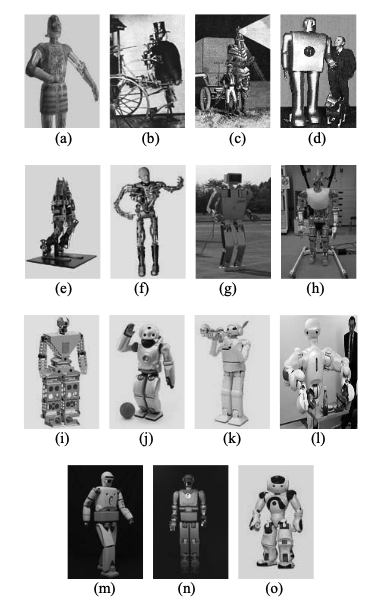
\includegraphics[scale=1.0]{images/intro-3.png}\hfill
    \caption[Humanoid robots over decades]{Some Bipedal Android robots over decades \cite{evolution} 
        (a) First humanoid robot by Leanardo Da vinci (b) Steam Mam in 1865 (c) Electric man in 1885 (d) 
        ELEKTRO in 1938 (e) BIPER - 4 in 1984 (f) Tron-XM in 1997 (g) H6 Humanoid robot in 2000 (h) Robot 
        JACK in 2000 (i)  GuRoo in 2002 (j) QRIO, Sony in 2003 (k) Partnar Robot, Toyoto in 2004 (l) TwentyOne
        in 2007 (m) REEM-A in 2007 (n) REEM-B in 2008 (o) NAO in 2008.}\hfill
    \label{humanoid-robots}
\end{figure}

The idea of building machines which look and move like humans has been explored by philosophers and mathematicians
since antiquity. Nowadays, the concepts of such machines are a part of research in robotics. Humanoid robots can 
be thought of as mechanical, actuated devices that can perform human-like manipulation, including locomotion as 
their main skill for displacement. Well before the first modern humanoid robot, one of the biggest steps towards 
this objective was achieved in 1956 with the first commercial robot manipulator, \textit{Unimate, from Unimation}. 
The automotive industry was the first to benefit from these kinds of manipulator robots. Recently, the development 
of humanoid robots for education, research and services has proved the work in multiple ways. 

 

Current goals of research in humanoid robots include industrial and social applications in day-to-day life. 
A study was conducted by Tanie, \cite{tanie} and is briefed below

\begin{itemize}
\item maintenance tasks of industrial plants,
\item security service for home and offices,
\item human care, teleoperation of construction machines.
\item cooperative work
\end{itemize}

Since many studies have explored this aspect of robot motion and how to make robots more \textit{human-like} and 
\textit{human-aware}. Human Robot Interaction (HRI) is now a challenging research field and studies on the efficacy 
of humanoid robots in human environments are further proceeded.

\section{Measuring Human Movement}

Kinesiology is defined as the scientific study of human movement. To access human motion, Kinesiology involves principles
and methods from \textit{biomechanics, anatomy, physiology and motor learning}. Its range of application includes health
promotion, rehabilitation, ergonomics, health and safety in industry, disability management, among others. The 
measurement of human movement is one of the tools that is central in this research field. In 19th century, various 
devices were built to produce the moving pictures, among those exists the most advanced technique named 
\textit{chronophotography}. This device allowed to study fast paced human motions by recording and reproducing the 
captured motion \cite{RosenhahnBodo2008HMUM}. Another major contribution in motion study is the study on the path of 
center of mass during human displacement \cite{alma991010593879705596}.

 

\begin{figure}[h!]
\centering
% \captionsetup{justification=centering,margin=2cm}
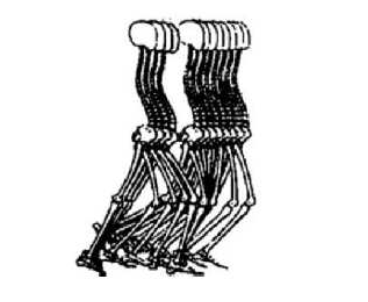
\includegraphics[scale=0.4]{images/intro-2.png}\hfill
\caption[Human Locomotion using Differential Equations]{Computation of human locomotion using differential equations by Weber Brothers \cite{alma991010593879705596}. The coordination between arms and legs was observed clearly.}\hfill
\label{motion-coordination}
\end{figure}

The first experimental studies of human gait \cite{alma991010593879705596}, i.e. determining physical quantities 
like inertial properties, were conducted by Christian W. Braune (1831-1892) and Otto Fischer(1861-1917). They 
considered the human body as rigid bodies in form of dynamic links in series. The work of Nicholas Bernstein (1896-1966)
in Moscow introduced the 3D analysis based on cameras. The methods for measuring human movement continued improving 
with the advent of new technologies like electronics and magnetic devices, up until today’s motion capture systems 
based on reflective markers, magnetic or inertial devices. Recently, there has been a huge development in the motion 
capture systems which evolved the motion study to newer dimensions (discussed in the later chapter).

\section{Challenges in Motion Imitation}

Given the resemblance between humanoid robots and human beings, it is natural to look for inspiration in human movements
in order to generate motion for the humanoid. The most straightforward way is to have the robot observe what the human 
does and reproduce that behaviour, i.e. perform imitation. After all, even human beings themselves are able to acquire 
skills by imitation and learning.

\begin{figure}[h!]
\centering
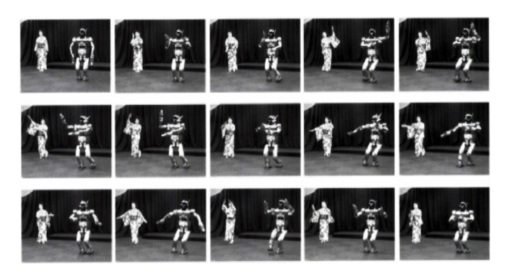
\includegraphics[scale=0.9]{images/motion-imitation.png}\hfill
\caption[A motion imitation performance by HRP-2 humanoid robot]{A performance  based on motion imitation done by 
HRP-2 humanoid robot}\hfill
\label{marker-based-system}
\end{figure}


If humanoid robots are to interact with human beings, it is imperative that their gestures are human-like since much of
human communication is non-verbal. Programming each aspect of the motion detail by detail in order to make it human-like
is time-consuming and not fit to handle the immense variety and complexity of human behaviours. Thus, imitation comes
as a more natural and intuitive alternative to classical methods, since more information can be transmitted directly.

 

Human motion cannot be directly transferred to the robot without choosing beforehand which affects the ocean or what
is transferring. The most advanced human robots cannot move completely like a human being. The robots are limited 
by differences to human counterparts such as the number of degrees of freedom, link lengths, motor torques, etc. 
Robots which tried to reproduce the whole human body inevitably have never taken dynamic differences from the human 
body they are trying to represent.

 

While performing imitations, the physical differences have to be taken into account when mapping the register home 
movements to the robot morphology. This was addressed by Pollard et al. [5], who limited the captured human motion 
to a range achievable by the robot by locally scaling angles and velocities in order to preserve as much as possible 
local variations in the motion imitated by the Sarcos robot.


\section{Problem Statement}

Recently, almost every humanoid robots are able to walk and balance in flat indoor environments and there are robots 
proved walking on rugged terrains and uneven planes are possible and achievable. A lot of effort is being done to make
them more autonomous by incorporating the perception, planning and action loop. One of the ultimate objective of the 
humanoid robot, as mentioned before is to create the humanoid motion more human-precise. In this sense, robots require 
real-time imitation processed be higher reactivity compensating the unpredictable nature of human motion.

 

In humans, imitation is an advanced behavior whereby an individual observes and replicates the action of another 
human arguably with more accuracy and precision. However in humanoid robots, these kind of motion imitations are possible
up to kinematic level through perception; the robot can also be able to imitate the action posture dynamically using its predefined 
configurations and controllers to an extent. But for a complete imitation at dynamic level, humanoid robots are still struggling to 
approximately copy the dynamic parameters applied during the action. Presently, to copy the action at dynamic level, 
feedback data from human during motion or action is mandatory. The motion data from human action is transferred using 
\textit{Xsens MVN Analyze}. The main objective of the thesis is to define realtime dynamic balance constraint during
motion imitation and validate it experimentally using an affordable humanoid robot, \textit{NAO} from \textit{Aldebaran
Robotics}. The balancing constraint of the robot is controlled using an Hierachical Quadratic Programming (HQP) and validated on both 
simulation and real robot.

\section{Thesis Organisation}


The chapters of the thesis are organized as follows. Chapter \ref{chapter-2} introduces the generalities of humanoid robotics and presents
the state of the art in the control and balance of this type of robots. The existing works on motion retargetting involving dynamics are also 
discussed. Chapter \ref{chapter-3} presents the mathematical requirements for the motion imitation problem. The approaches for CoM and ZMP
retargetting are also explained in this chapter. Posture Control during motion imitation using multiple double inverted pendulums are proposed.
Chapter \ref{chapter-4} presents the essential concepts of hierrachical quadratic programming (HQP) and presents the tuned approach for
retargetting problem. Chapter \ref{chapter-5} describes the environmental setup of the proposed system. Information on Xsens and NAOqi are 
detailed in this chapter. Chapter \ref{chapter-6} details the implementation of HQP and their corresponding results. The final chapter 7 
concludes the overall work, discussion and the future scope of the thesis.